%%%%%%%%%%%%%%%%%%%%%%%%%%%%%%%%%%%%%%%%
%% MCM/ICM LaTeX Template %%
%% 2021 MCM/ICM           %%
%%%%%%%%%%%%%%%%%%%%%%%%%%%%%%%%%%%%%%%%
\documentclass[12pt]{article}
\usepackage{geometry}
\geometry{left=1in,right=0.75in,top=1in,bottom=1in}

%%%%%%%%%%%%%%%%%%%%%%%%%%%%%%%%%%%%%%%%
% Replace ABCDEF in the next line with your chosen problem
% and replace 1111111 with your Team Control Number
\newcommand{\Problem}{D}
\newcommand{\Team}{2100545}
%%%%%%%%%%%%%%%%%%%%%%%%%%%%%%%%%%%%%%%%

\usepackage{newtxtext}
\usepackage{amsmath,amssymb,amsthm}
\usepackage{newtxmath} % must come after amsXXX

\usepackage[pdftex]{graphicx}
\usepackage{xcolor}
\usepackage{fancyhdr}
\lhead{Team \Team}
\rhead{}
\cfoot{}
\setlength{\parskip}{1em}


\newtheorem{theorem}{Theorem}
\newtheorem{corollary}[theorem]{Corollary}
\newtheorem{lemma}[theorem]{Lemma}
\newtheorem{definition}{Definition}

%%%%%%%%%%%%%%%%%%%%%%%%%%%%%%%%
\begin{document}
\graphicspath{{.}}  % Place your graphic files in the same directory as your main document
\DeclareGraphicsExtensions{.pdf, .jpg, .tif, .png}
\thispagestyle{empty}
\vspace*{-16ex}
\centerline{\begin{tabular}{*3{c}}
	\parbox[t]{0.3\linewidth}{\begin{center}\textbf{Problem Chosen}\\ \Large \textcolor{red}{\Problem}\end{center}}
	& \parbox[t]{0.3\linewidth}{\begin{center}\textbf{2021\\ MCM/ICM\\ Summary Sheet}\end{center}}
	& \parbox[t]{0.3\linewidth}{\begin{center}\textbf{Team Control Number}\\ \Large \textcolor{red}{\Team}\end{center}}	\\
	\hline
\end{tabular}}
%%%%%%%%%%% Begin Summary %%%%%%%%%%%
% Enter your summary here replacing the (red) text
% Replace the text from here ...

\begin{center}
\textbf{Music change the world}\\
Use this template to begin typing the first page (summary page) of your electronic report. This \newline
template uses a 12-point Times New Roman font. Submit your paper as an Adobe PDF \newline
electronic file (e.g. 1111111.pdf), typed in English, with a readable font of at least 12-point type.	\\[2ex]
Do not include the name of your school, advisor, or team members on this or any page.	\\[2ex]
Papers must be within the 25 page limit.	\\[2ex]
Be sure to change the control number and problem choice above.	\\
You may delete these instructions as you begin to type your report here. 	\\[2ex]
\textbf{Follow us @COMAPMath on Twitter or COMAPCHINAOFFICIAL on Weibo for the \newline
most up to date contest information.}

\end{center}

% to here
%%%%%%%%%%% End Summary %%%%%%%%%%%

%%%%%%%%%%%%%%%%%%%%%%%%%%%%%%
\clearpage
\pagestyle{fancy}
% Uncomment the next line to generate a Table of Contents
%\tableofcontents 
\newpage
\setcounter{page}{1}
\rhead{Page \thepage\ }
%%%%%%%%%%%%%%%%%%%%%%%%%%%%%%
\title{Music changes the world}
\maketitle
\tableofcontents
\section{Introduction}
\subsection{Background}
\begin{itemize}
\item The evolutionary trajectory and intrinsic interactions of western popular music
\end {itemize}\quad \quad
Nowadays, it has become a more and more common phenomenon for people to listen to all kinds of music to seek pleasure and relax themselves. And we may abstract and conclude the invariable key elements in the forever-changeable styles and contents of music. That are melody, harmony, lyrics, rhythm, and timbre, etc. And in analysing the similarity and developmental portraits among some of these elements, we may have a primary clue on how the previous musicians have exerted their influence upon their same and subsequent generations of musicians and give some insights into how a new genre of music came into being.\par
Utilizing the interactive network model, we are able to implement the cross-tabulation of the various specimens given, and further explore the deep-rooted relationship between different musicians over time, therefore produce a elementary work on the evolutionary trajectory of music.

\subsection{Restatement of the problem}\quad \quad
From the data we retrieved.\cite{1} We can learn that all the artist in the world has their influences. Not only to the genre of music he specialized. But also to some specific artists from the younger generation. Our first mission is to create a network that links the influencer and the follower. Through the network,we may find the indicators of "musical influence". The weight and the form of the network can show us the relationship between different artists. They may be influencers, or followers. Or they can be both.\par
Similarity is also an index we focus to. Since there are experts already defined some features and factors of musical compositions. Features such as danceability, energy or liveness is hard to define by amateurs like us. However, the expert quantized these features so we can process them easily. In this case, we should find out that the similarity between artists from the same genre or from different genres.\par
The revolution of music through a period of time is also an significant argument we are facing. Each artists is active in different eras. Thus only the artists who became active earlier can influence the latter artists. Each era has their favorites, how does people's taste varies is also an interesting problem to solve.\par
In short, we can divide the whole task into the following parts.
\begin{itemize}
\item Build the network that can show us the relationship between artists: who is the influencer and who is the follower.
\item Take the time and genre into consideration. Find out how these indicators affect our model.
\item Use our model and analyze the data we processed. After all, we can have our own thoughts about it. How does music affect the society? And how much is the influence of a revolutionary artist/genre.
\end{itemize}
Our model is meant to figure out the intrinsic information from the data we already knew. By processing the data with our model,we can learn a lot of hidden information. Hence we can answer the questions like: who is the major influencer of an era and how he led the popularity, which genre of music is the most popular one, how does the fashion changes over time. At last, we may even find out which genre will lead the major revolution of music.
\subsection{notation}

\section{Analysis of the Problem}
The directed influential network of influencer-artists and their followers can be built in this way: First, in order to take better advantage of the whole influence data set, we (choose a thousand pieces randomly from the 42771 pieces of given influence data, ) and use each node to represent an artist, we also assign different genres of artists with different colors to better distinguish them. The node's arc goes from the influencer to the follower, in this case, we can observe what are the nodes that points to a particular node (the node's in-degree) to see the amount and genres of artists that have influenced this particular artist, in the same way, by observing what nodes are a particular node pointing to, (the node's out-degree), we can gain knowledge about the amount and genres of artists that this particular artist have influenced.
\begin{figure}[h]
\small
\flushleft
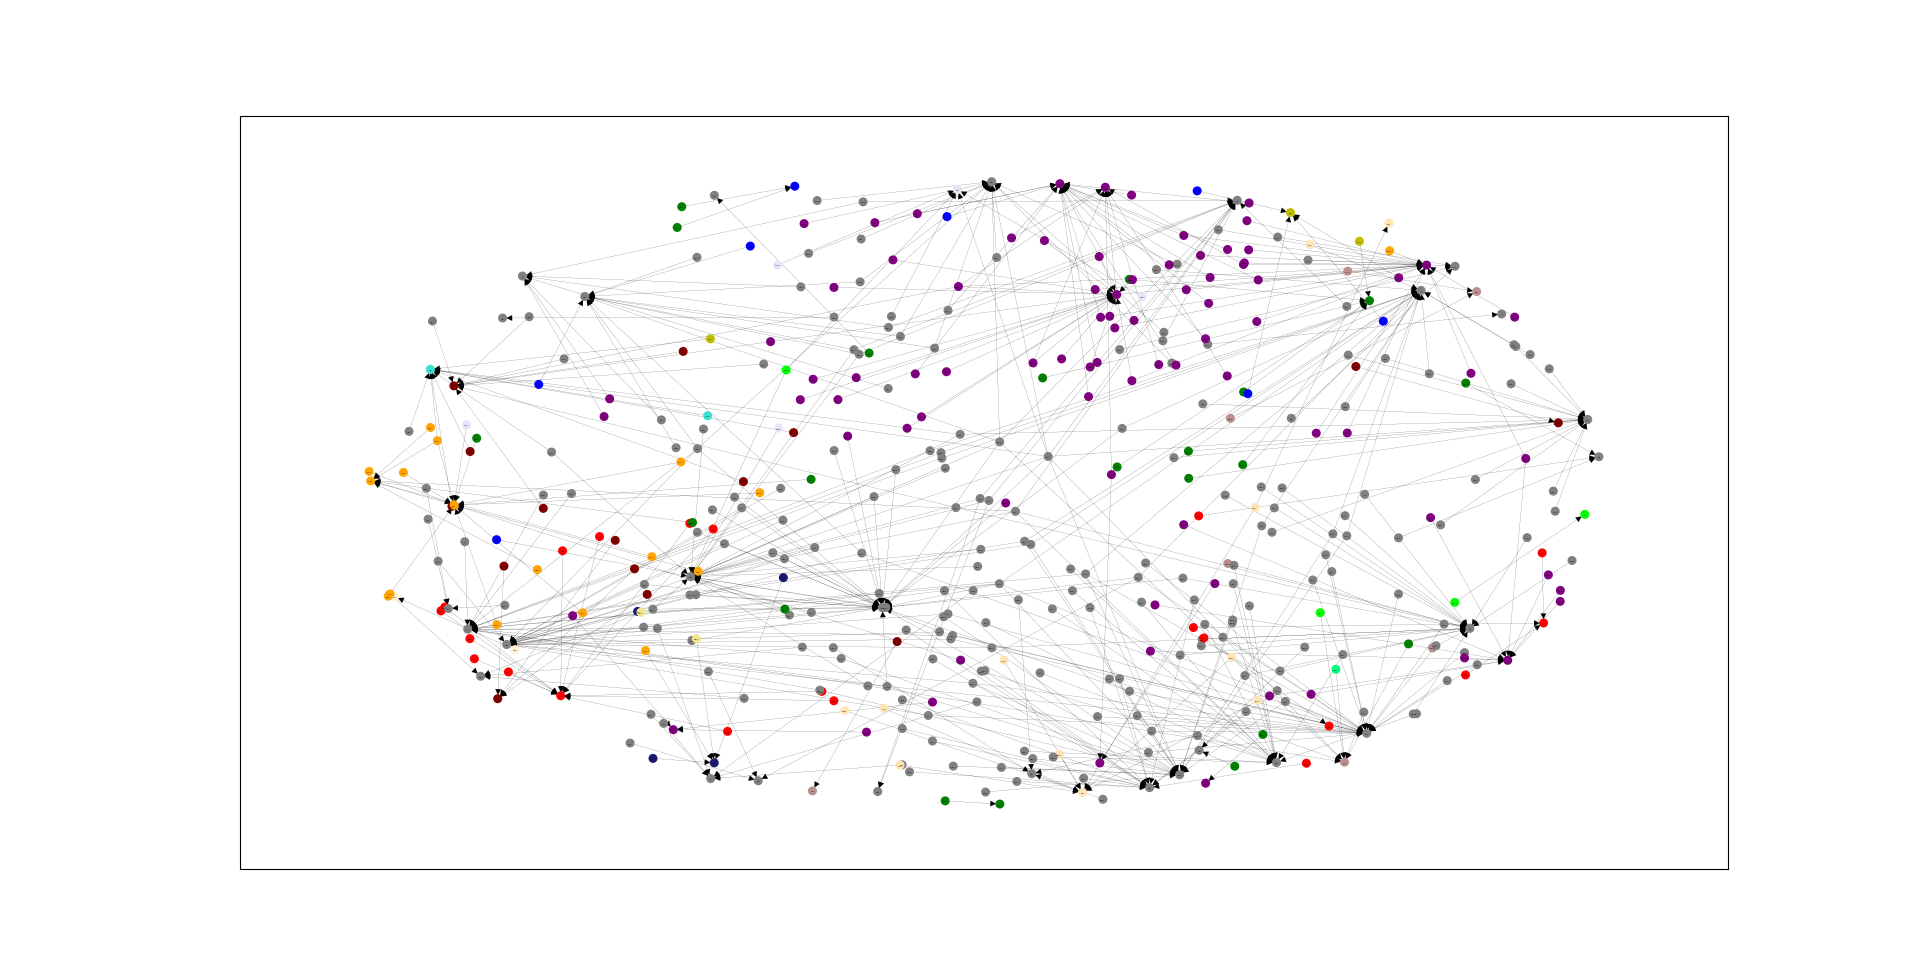
\includegraphics[width=19cm]{firstmodel.png}
\caption{network of influencer-artists and their followers}
\end{figure}
\begin{center}
\begin{tabular}{l|l}
Color & Genres of artists
\\ \hline
Pop/Rock  & grey       \\                     
R \& B  & purple\\
Country & red\\
Jazz & green\\
Vocal & orange\\
Blues & blue\\
Folk & khaki\\
Reggae & moccasin\\
Electronic & rosybrown\\
Latin & maroon\\
International & y\\
Religious & navy\\
Stage \& Screen & lavender\\
Comedy/Spoken & midnightblue\\
Classical & lime\\
New Age & papayawhip\\
Avant-Garde & springgreen\\
Easy Listening & turquoise\\
Children\' s & azure\\
Unknown & teal\\
influencer\_main\_genre & violet\\
\end{tabular}
\end{center}
\begin{figure}
\small
\centering
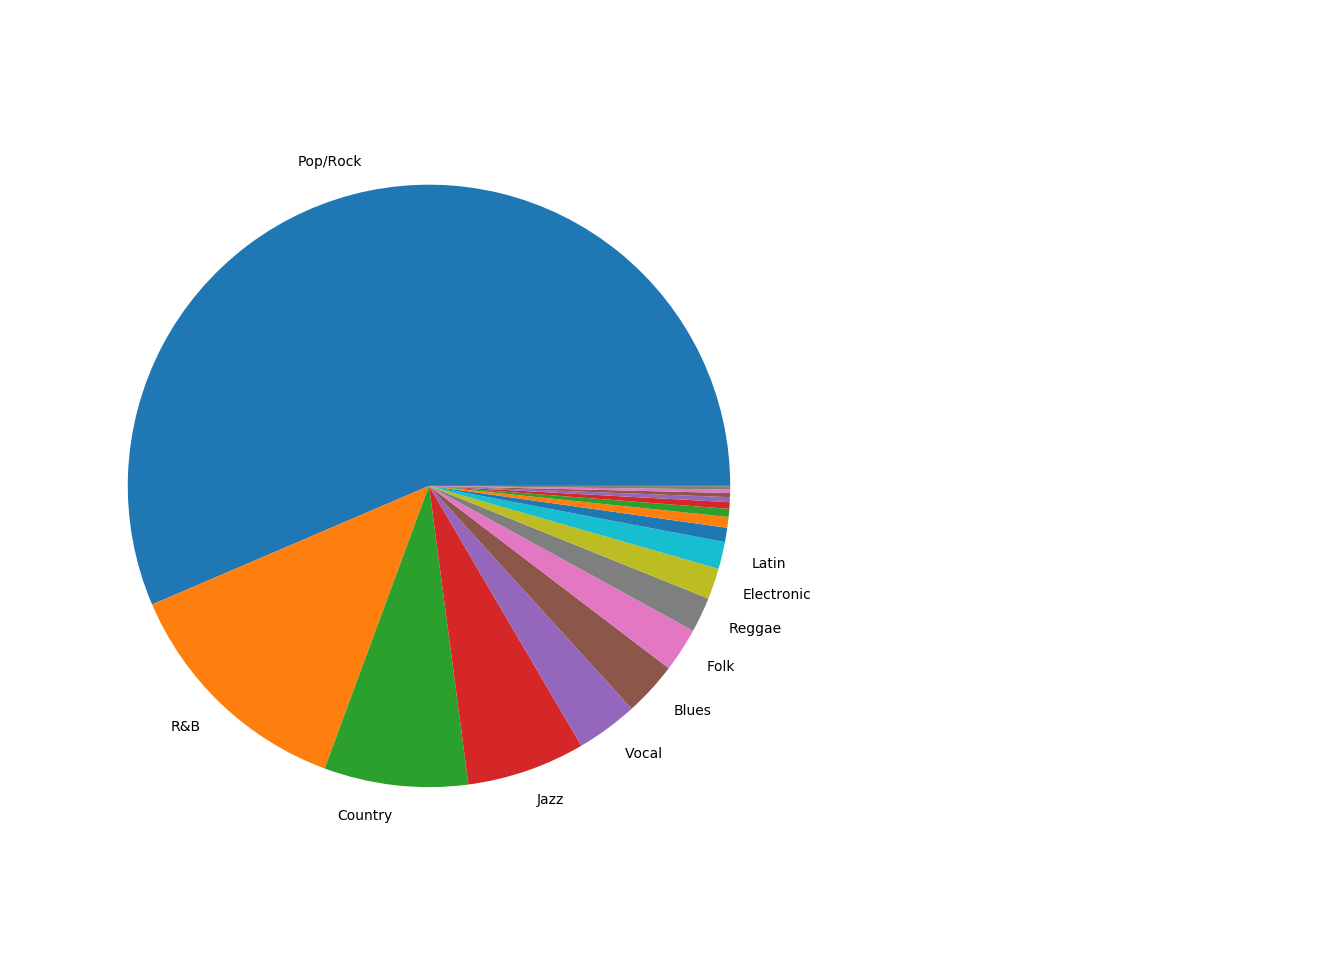
\includegraphics[width=24cm]{Figure_1.png}
\caption{The proportion of each genre}
\end{figure}


%%%%%%%%%%%%%%%%%%%%%%%%%%%%%%
\end{document}
\end
